\documentclass[a4paper]{jarticle}

\usepackage{moreverb}
\usepackage{ascmac}
\usepackage{eclbkbox}
\usepackage[dvipdfmx]{graphicx}

\setlength{\textheight}{\paperheight}   % 紙面縦幅を本文領域にする(BOTTOM=-TOP)
\setlength{\topmargin}{4.6truemm}       % 上の余白を30mm(=1inch+4.6mm)に
\addtolength{\topmargin}{-\headheight}  % 
\addtolength{\topmargin}{-\headsep}     % ヘッダの分だけ本文領域を移動させる
\addtolength{\textheight}{-60truemm}    % 下の余白も30mm(BOTTOM=-TOPだから+TOP+30mm)

\setlength{\textwidth}{\paperwidth}     % 紙面横幅を本文領域にする(RIGHT=-LEFT)
\setlength{\oddsidemargin}{-0.4truemm}  % 左の余白を25mm(=1inch-0.4mm)に
\setlength{\evensidemargin}{-0.4truemm} % 
\addtolength{\textwidth}{-50truemm}     % 右の余白も25mm(RIGHT=-LEFT)

\begin{document}
\title{パタン認識特論\\第1回レポート課題}
\author{3G150131 松井 健人}
\date{2015年5月20日}
\maketitle

%-----------------------------
%1章
%-----------------------------

\section{課題}
教科書「わかりやすいパターン認識(オーム社)」の「{2.3} パーセプトロンの学習規則」の内容に従って,{1}次元データ(図{2.4})に対するパーセプトロンの計算を実行し,{23}ページの図{2.7}を作図せよ.計算に用いる言語はJavaかCとする.\\
\\提出物:\\ 
{\textcircled{\scriptsize 1}}.作成したプログラムソースコードを印刷したもの.\\
{\textcircled{\scriptsize 2}}.作図結果($\rho$の値を{1.2}と{2.0},{3.6}に設定した係数ベクトルの変化パタンを{3}種).\\
※提出物の様式は自由.但し,学籍番号と氏名は忘れずに!!\\
提出期限:2015年5月20日.
提出先:恵喜館の片桐のメールボックス.

%-----------------------------
%2章
%-----------------------------

\section{パーセプトロンの学習規則}\label{perceptron}
パーセプトロンの学習規則とは,線形識別関数の重みを学習によって決定する方法である.
パーセプトロンの学習規則の手順を以下に示す.

\begin{enumerate}
\renewcommand{\labelenumi}{(\arabic{enumi})}
\item 重みベクトル\mbox{\boldmath $w$}の初期値を適当に設定する.
\item $\chi$の中から学習パターンを1つ選ぶ.
\item 識別関数$g(x)=$\mbox{\boldmath $w$}$^{T}$\mbox{\boldmath $x$}によって識別を行い,正しく識別できなかった場合のみ次のように重みベクトル\mbox{\boldmath $w$}を修正し,新しい重みベクトル\mbox{\boldmath $w'$}を作る.
\begin{equation}
\mbox{\boldmath $w'$}=\mbox{\boldmath $w$}+\rho・\mbox{\boldmath $x$}  (\omega_{1}のパターンに対してg(x) \leq {0}となったとき)
\end{equation}
\begin{equation}
\mbox{\boldmath $w'$}=\mbox{\boldmath $w$}-\rho・\mbox{\boldmath $x$}  (\omega_{2}のパターンに対してg(x) \geq {0}となったとき)
\end{equation}
\item 上の処理(2),(3)を{$\chi$}の全パターンに対して繰り返す.
\item  {$\chi$}の全パターンを正しく識別できたら終了.誤りがあるときは(2)に戻る.
\end{enumerate}

%-----------------------------
%3章
%-----------------------------

\newpage
\section{作成したプログラムソースコード}\label{program}
\ref{perceptron}章で示したパーセプトロンの学習規則をJavaを用いて作成した.
2つのクラス$\omega_1$,$\omega_2$が存在し,それぞれに学習パターンが3つずつ属している.
$\omega_1$に属する学習パターンは,$(x_1, x_2, x_3) = (1.2, 0.2, -0.2)$であり,
$\omega_2$に属する学習パターンは,$(x_4, x_5, x_6) = (-0.5, -1.0, -1.5)$である.
この学習パターンを基に,$\rho$の値を{1.2},{2.0},{3.6}に設定し,重みベクトル\mbox{\boldmath $w$}をそれぞれ$(w_1, w_0) = (2,-7)$,$(w_1, w_0) = (5,11)$,$(w_1, w_0) = (2,-7)$として計算を行った.
ソースコードをリスト 1に示す.また,出力結果をリスト 2に示す.


\vspace{3mm}
\begin{center}
リスト 1: プログラムソースコード
\begin{small}
\vspace{3mm}
\listinginput{1}{PerceptronConvergenceTheorem_edit2.java}
\end{small}
\vspace{3mm}
\end{center}

\newpage
\begin{center}
リスト 2: 出力結果
\begin{small}
\vspace{3mm}
\begin{breakbox}
\verbatimtabinput{result.txt}
\end{breakbox}
\end{small}
\end{center}

%-----------------------------
%4章
%-----------------------------
\newpage
\section{作図結果}
\ref{program}章に示したプログラムにより計算した重みベクトルの遷移をExcelを用いて作図した結果を図\ref{graph}に示す.
\begin{figure}[!h]
  \centering
  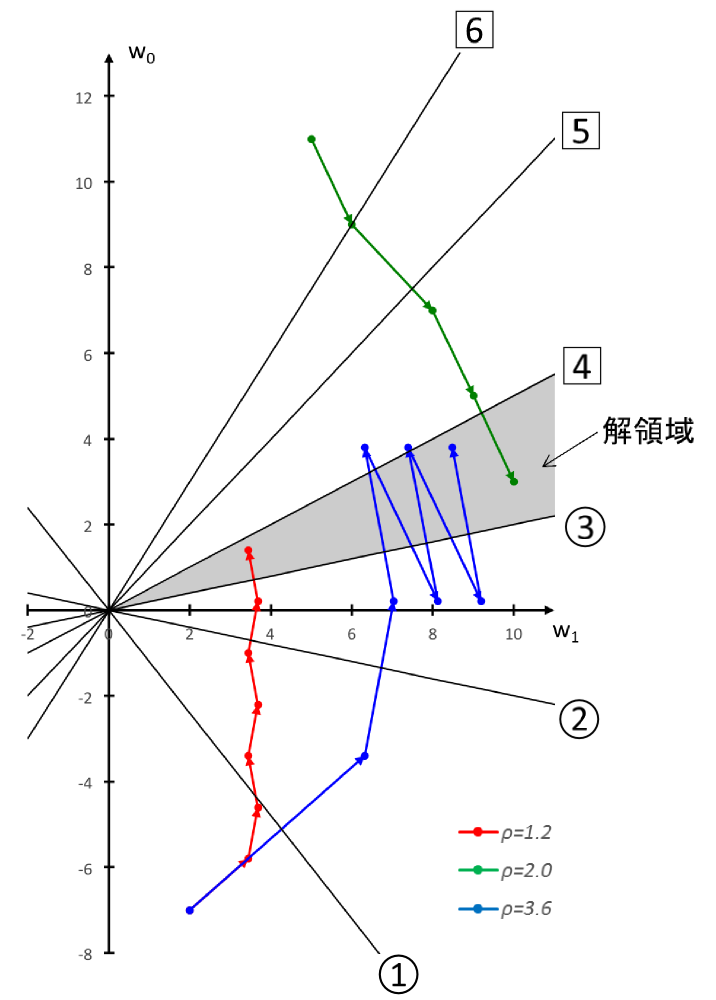
\includegraphics[height=20cm]{graph2.png}
  \caption{重みベクトルの遷移}
 \label{graph}

\end{figure}


\end{document}